\chapter{Model Validation}\label{ch:modValPerf}

\todo[color=06modelValidationAndPerformance]{Model Validation and Performance}
To validate the model acquired in Chapter \ref{ch:mathmodel}, we ran a second test with the 
same setup as described in Chapter \ref{ch:experiment}. Coefficients were determined for pump models,
for every percentage of the valve opening.

Equation \ref{eq:pumpHeadModel60} and \ref{eq:pumpPowerModel60} represent the modeled Flow and Power 
Consumption for 60 \% pump speed.

\begin{equation}
	H(\omega) = \frac{\bar{a_0}}{\bar{\omega_0^2}} \cdot \omega^2 + \frac{\bar{a_1}}{\bar{\omega_0}} \cdot \omega \cdot Q(\omega) + \bar{a_2} \cdot Q(\omega)^2
	\label{eq:pumpHeadModel60}
\end{equation}
\begin{equation}
	P(\omega) = \frac{\bar{b_0}}{\bar{\omega_0^3}} \cdot \omega^3 + \frac{\bar{b_1}}{\bar{\omega_0^2}} \cdot \omega^2 \cdot Q(\omega) + \frac{\bar{b_2}}{\omega_0} \cdot \omega \cdot Q(\omega)^2 + b_3 \cdot Q(\omega)^3
	\label{eq:pumpPowerModel60}
\end{equation}

The coefficients for the model were determined at 60 \% pump speed and can be seen below.

\begin{align*}
	\bar{a_0} = -0.03044 && \bar{a_1} = 0.07635  && \bar{a_2} = 1.688  \\
	\bar{b_0} = -0.2825 && \bar{b_1} = -0.7147 && \bar{b_2} = 54.39 && \bar{b_3} = 163.7 \\
	\bar{\omega_0} = 2298 rpm \\
\end{align*}
\newpage
Figures \ref{fig:flowVsModeledPressure} and \ref{fig:flowVsModeledPower}, represent the Pressure and 
the Power Consumption for one of the tests.

\begin{figure}[ht]
	\centering
	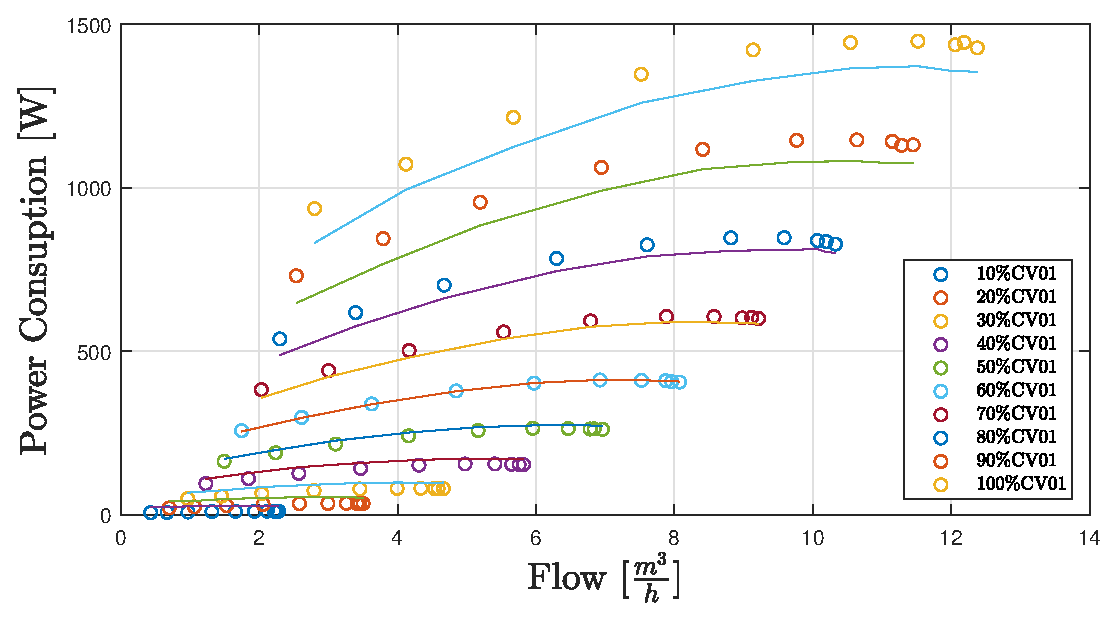
\includegraphics[width=0.8\textwidth]{figures/06ModelValidation/flowVsModeledPowerConsumption.eps}
	\caption{Flow Vs. Modeled Power Consumption}
	\label{fig:flowVsModeledPower}
\end{figure}
\begin{figure}[ht]
	\centering
	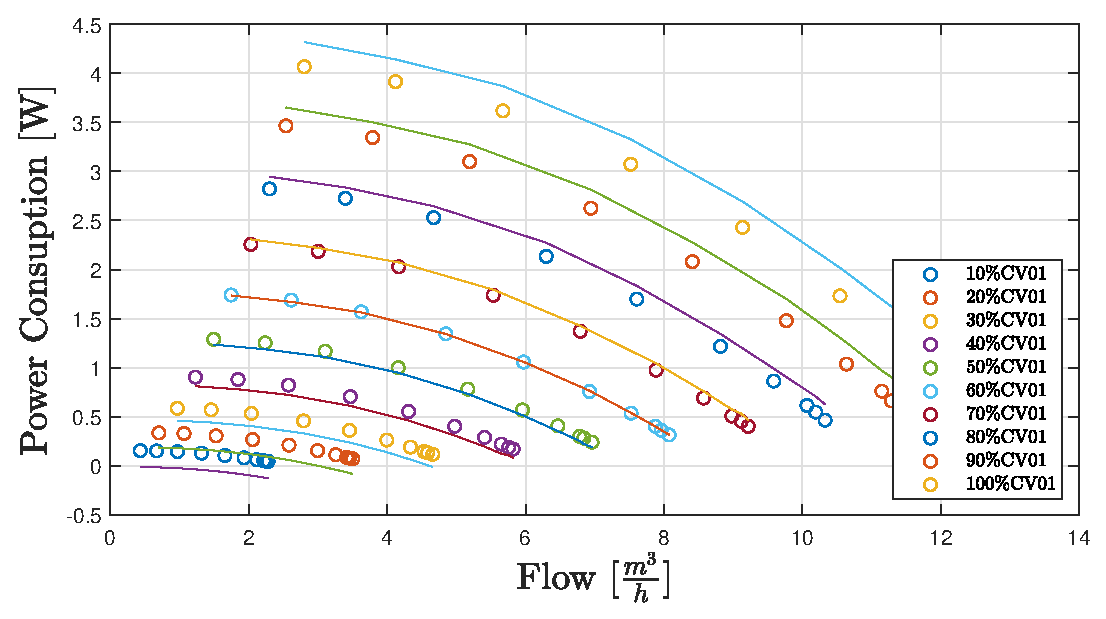
\includegraphics[width=0.8\textwidth]{figures/06ModelValidation/flowVsModeledPressure.eps}
	\caption{Flow Vs. Modeled Pressure}
	\label{fig:flowVsModeledPressure}
\end{figure}

As expected, the models are able to approximate the pump curves, that are closer to the actual pump speed 
the models were determined for. They are not as accurate overall as expected. 
The modelling errors could come as a result of many factors, however, there is room for improvement. 
As with the case of the pressure sensors, we were not able to determine accurate values for 
the pump speeds. Again, we have used gains and offsets provided to us. Additionally, as stated in [X]
motor and drive efficiency are not accounted for.
\todo[color=06modelValidationAndPerformance]{quote zhenyu paper}
\newpage
Other modelling errors, could be introduced by the manner in which the models were determined. The data we
used was processed in such a manner that only average values over a period of time were used.
\todo[color=06modelValidationAndPerformance]{maybe new section}

A better approach, would have been to model the whole range of values. We have done this, but it turned out unsuccessfully. 
The computing power was simply not enough.
The simulation was ran for 15 seconds each time the pump speed was changed. If instead, the simulation had been ran for
10 seconds, the data would have been less, but this might have not been enough for the Pressure and Flow to reach a 
steady state.